\documentclass[main.tex,fontsize=8pt,paper=a4,paper=portrait,DIV=calc,]{scrartcl}
% Document
\usepackage[T1]{fontenc}
\usepackage[dvipsnames]{xcolor}
\usepackage[nswissgerman,english]{babel}
\renewcommand{\familydefault}{\sfdefault}

% Format
\usepackage[top=5mm,bottom=1mm,left=5mm,right=5mm]{geometry}
%\setlength{\headheight}{\baselineskip}
%\setlength{\headsep}{0mm}

%\usepackage{scrlayer-scrpage}
%\clearpairofpagestyles
%\chead{{\bfseries\TITLE, \AUTHOR, \pagename~\thepage}}

%\addtokomafont{pagehead}{\upshape}

\usepackage{multicol}
\setlength{\columnsep}{2mm}
\setlength{\columnseprule}{0.1pt}

% Math
\usepackage{amsmath}
\usepackage{amssymb}
\usepackage{amsfonts}

% Code
\usepackage{fancyvrb, etoolbox, listings, xcolor}
%\usemintedstyle{bw}

%\newminted[shell]{bash}{
%fontsize=\footnotesize,
%fontfamily=tt,
%breaklines=true,
%frame=single,
%framerule=0.1pt,
%framesep=2mm,
%tabsize=2
%}
%\newminted{css}{
%breaklines=true,
%tabsize=4,
%autogobble=true,
%escapeinside=||,
%stripall=true,
%stripnl=true,
%}

    \definecolor{lightgray}{rgb}{0.95, 0.95, 0.95}
    \definecolor{darkgray}{rgb}{0.4, 0.4, 0.4}
    \definecolor{purple}{rgb}{0.65, 0.12, 0.82}
    \definecolor{ocherCode}{rgb}{1, 0.5, 0} % #FF7F00 -> rgb(239, 169, 0)
    \definecolor{blueCode}{rgb}{0, 0, 0.93} % #0000EE -> rgb(0, 0, 238)
    \definecolor{greenCode}{rgb}{0, 0.6, 0} % #009900 -> rgb(0, 153, 0)
    \definecolor{teal}{rgb}{0.0, 0.5, 0.5}

\lstdefinestyle{code}{
    identifierstyle=\color{black},
    keywordstyle=\color{blue}\bfseries\small,
    ndkeywordstyle=\color{greenCode}\bfseries\small,
    stringstyle=\color{ocherCode}\ttfamily\small,
    commentstyle=\color{teal}\ttfamily\textit\small,
    basicstyle=\ttfamily\small,
    breakatwhitespace=false,         
    breaklines=true,                 
    captionpos=b,                    
    keepspaces=true,                 
    showspaces=false,                
    showstringspaces=false,
    showtabs=false,                  
    tabsize=2,
    belowskip=-5pt
}



% Images
\usepackage{graphicx}
\newcommand{\pic}{\includegraphics[scale=0.3]}
\graphicspath{{Screenshots/}{../Screenshots}}
\makeatletter
\def\pictext#1#2{%
    \@ifnextchar[{%
    \pictext@iiiii{#1}{#2}%
    }{%
      \pictext@iiiii{#1}{#2}[0.5,0.4,0.3]% Default is 5
    }%
}
\def\pictext@iiiii#1#2[#3,#4,#5]{\begin{minipage}{#3\textwidth}\includegraphics[scale=#4]{#1}\end{minipage}\begin{minipage}{#5\textwidth}#2\end{minipage}}
\def\minipg#1#2{%
    \@ifnextchar[{%
    \minipg@iiii{#1}{#2}%
    }{%
      \minipg@iiii{#1}{#2}[0.3,0.6]% Default is 5
    }%
}
\def\minipg@iiii#1#2[#3,#4]{\vspace{0.8mm}\begin{minipage}{#3\textwidth}#1\end{minipage}\begin{minipage}{#4\textwidth}#2\end{minipage}{\vspace{0.8mm}}}
\makeatother

%\newenvironment{minty}[2]% environment name
%{% begin code
%  \begin{minipage}{#1}
%  \begin{minted}{#2}
%}%
%{% end code
%  \end{minted}
%  \end{minipage}
%  \end{minty}\ignorespacesafterend
%} 

% Smaller Lists
\usepackage{enumitem}
\setlist[itemize,enumerate]{leftmargin=3mm, labelindent=0mm, labelwidth=1mm, labelsep=1mm, nosep}
\setlist[description]{leftmargin=0mm, nosep}
\setlength{\parindent}{0cm}

% Smaller Titles
\usepackage[explicit]{titlesec}

%% Color Boxes
\newcommand{\sectioncolor}[1]{\colorbox{black!60}{\parbox{0.989\linewidth}{\color{white}#1}}}
\newcommand{\subsectioncolor}[1]{\colorbox{black!50}{\parbox{0.989\linewidth}{\color{white}#1}}}
\newcommand{\subsubsectioncolor}[1]{\colorbox{black!40}{\parbox{0.989\linewidth}{\color{white}#1}}}
\newcommand{\paragraphcolor}[1]{\colorbox{black!30}{\parbox{0.989\linewidth}{\color{white}#1}}}
\newcommand{\subparagraphcolor}[1]{\colorbox{black!20}{\parbox{0.989\linewidth}{\color{white}#1}}}

%% Title Format
\titleformat{\section}{\vspace{0.5mm}\bfseries}{}{0mm}{\sectioncolor{\thesection~#1}}[{\vspace{0.5mm}}]
\titleformat{\subsection}{\vspace{0.5mm}\bfseries}{}{0mm}{\subsectioncolor{\thesubsection~#1}}[{\vspace{0.5mm}}]
\titleformat{\subsubsection}{\vspace{0.5mm}\bfseries}{}{0mm}{\subsubsectioncolor{\thesubsubsection~#1}}[{\vspace{0.5mm}}]
\titleformat{\paragraph}{\vspace{0.5mm}\bfseries}{}{0mm}{\paragraphcolor{\theparagraph~#1}}[{\vspace{0.5mm}}]
\titleformat{\subparagraph}{\vspace{0.5mm}\bfseries}{}{0mm}{\subparagraphcolor{\thesubparagraph~#1}}[{\vspace{0.5mm}}]

%% Title Spacing
\titlespacing{\section}{0mm}{0mm}{0mm}
\titlespacing{\subsection}{0mm}{0mm}{0mm}
\titlespacing{\subsubsection}{0mm}{0mm}{0mm}
\titlespacing{\paragraph}{0mm}{0mm}{0mm}
\titlespacing{\subparagraph}{0mm}{0mm}{0mm}

%% format cells
\usepackage[document]{ragged2e}
\usepackage{array, makecell}
\renewcommand{\arraystretch}{2}
\newcommand{\mc}{\makecell[{{m{1\linewidth}}}]}


\usepackage{listings-rust}

\lstset{
    language=Rust,
    style=colouredRust,
}
%%%%%

\begin{document}
\begin{table}[h!]
\section{Cargo}
\begin{tabular}{|m{0.2\linewidth}|m{0.755\linewidth}|}
\hline
Default Commands &
\vspace{2mm}
\begin{itemize}
  \item \textcolor{teal}{Cargo new} creates a new rust project with git integration
  \item \textcolor{teal}{Cargo build} build a project if the toml file has been provided
  \item \textcolor{teal}{Cargo build --release} builds the release version without debugging environment
  \item \textcolor{teal}{Cargo run} runs the project
  \item \textcolor{teal}{Cargo check} this only checks the code if it would compile! But it doesn't actually compile! Super helpful!
  \vspace{-3mm}
\end{itemize}\\
\hline
Toml & 
\begin{lstlisting}
[package]
name = "hello_cargo"
version = "0.1.0"
edition = "2021"

[dependencies]
\end{lstlisting}
\\
\hline
\end{tabular}
\section{Basic Terms and Information}
\begin{tabular}{|m{0.2\linewidth}|m{0.755\linewidth}|}
\hline
Comments & 
\textcolor{orange}{Comments are made with // just like C++ or C}\\
\hline
Main & 
\textcolor{orange}{Just like c++, the first function is always main!}\newline
\textcolor{teal}{However, unlike c++ the function definition order doesn't matter, there is no need for hpp files or similar!}\\
\hline
Naming convention & 
\vspace{2mm}
\begin{itemize}
  \item \textcolor{teal}{Functions: some\_function\_name()}
  \item \textcolor{teal}{}
  \item \textcolor{teal}{}
  \item \textcolor{teal}{}
  \vspace{-3mm}
\end{itemize}\\
\hline
\textbf{Macros} & 
\textcolor{orange}{You use a macro with the "!" keyword after a function}\newline
\begin{lstlisting}
fn main() {
    println!("Henlo birb!");
}
\end{lstlisting}\\
\hline
Variable definition & 
\textcolor{orange}{Rust has a peculiar syntax for writing variables, it is very much different to all other languages}\newline
\begin{lstlisting}
let num = 5; 
// this produces an immutable variable num, yes IMMUTABLE!!

let mut num2 = 5;
// num2 is MUTABLE because of the mut keyword!!

let mut num3: u32 = 5;
// this specifies a type of u32 int to the variable!
\end{lstlisting}\\
\hline
Strings & 
\textcolor{orange}{Strings in rust are strange, they are declared as follows:}\newline
\begin{lstlisting}
let mut grief = String::new();
// empty string

let mut grief = String::from("grief");
// mutable string with value "grief"
\end{lstlisting}
\, \newline
\textcolor{teal}{However, there are also trivial strings, they just do not have all the functions of the other strings.\newline
They do however in contrast work just like regular strings in c++.}\newline
\begin{lstlisting}
let mut str = "ping";
println!("{str}"); //prints ping
str += "pang";
println!("{str}"); //prints pingpang
\end{lstlisting}\\
\hline
Input \& Output & 
\begin{lstlisting}
std::io::stdin()
         .read_line(&mut num2)
         .expect("Failed to read line");
// the &mut is needed to reference the num2 variable as a mutable reference
// This string has by default an added newline,
// to get rid of this we have to format it
let num2 = num2.trim();
// this will create a new num2 variable and ghost the last one!!!
// .trim() will remove all whitespaces at the front and at the back
// just like definition it is by default immutable
// expect will trigger if the input has failed

// interesting is also the printing of variables inside println!
println!("The number is {num2}")
println!("The number is {},num2")
// these are identical! 
// If you have multiple numbers you have to order them in the same way as the empty {} are.
\end{lstlisting}
\, \newline
\textcolor{orange}{Similar to C++ we need namespaces to use standard library functions}\newline
\textcolor{teal}{.read\_line() has a result of either "Ok", or "Err" which must be handled with the .expected() function! \newline
This apparently will (guess) throw an error}\\
\hline
\end{tabular}
\end{table}
\pagebreak
\begin{table}[ht!]
\begin{tabular}{|m{0.2\linewidth}|m{0.755\linewidth}|}
\hline
conditional on Input & 
\textcolor{orange}{Instead of just parsing a string,\newline
we can also use functions on fail or ok states!}\newline
\begin{lstlisting}
loop {
    let mut guess = String::new();
    std::io::stdin()
        .read_line(&mut guess)
        .expect("failed to read line")
    
    let guess: u32 = match guess.trim().parse() { // match the parsed string
        Ok(num) => num, // if the string is a u32 int, then create the var num with that value
        Err(_) => continue, // continue the loop if it is not a u32 int
    }

}
\end{lstlisting}\\
\hline
loops & 
\textcolor{orange}{The easiest but also silliest loop in rust is the simple keyword: \textbf{loop}, it creates an infinite loop!}\newline
\begin{lstlisting}
loop {
    println!("I will print ping pang until you close the program!");
}
\end{lstlisting}\\
\hline
comparisons & 
\textcolor{orange}{Rust allows for a strange comparison syntax:}\newline
\begin{lstlisting}
loop {
    match guess.cmp(&secret_number) {
        Ordering::Less => println!("Too small!"), // do if guess is smaller
        Ordering::Greater => println!("Too big!"), // do if guess is bigger
        Ordering::Equal => { // do if guess is same!
            println!("You win!");
            break; // break loop
        }
    }
}
// Theoretically this is the same as a bunch of if-statements,
// however, I have no idea how the performance compapres....
\end{lstlisting}\\
\hline
random numbers & 
\textcolor{orange}{Unlike C or C++ you do not need to provide a seed.\newline
Just like in python you can simply use the rand function:}\newline
\begin{lstlisting}
let secret_number = rand::Rng::treadh_rng().gen_range(1..=100);
// this creates a rnadom number with range 1 to and with 100.
\end{lstlisting}\\
\hline
Constants & 
\begin{lstlisting}
cont SOME_CONSTANT: u32 = 5;
\end{lstlisting}\\
\hline
Scopes and Shadowing & 
\textcolor{orange}{Just like c++, when we have scopes and we redefine a variable, then it will only overwrite said variable in that scope.}\newline 
\begin{lstlisting}
let x = 5;
{ // empty scope
    let x = 10;
    println!({&x});
    // prints 10
}
println!({$x});
// prints 5
\end{lstlisting}
\, \newline
\textcolor{teal}{Interesting to know, you can create another variable with a different type and the same name!\newline 
This will still just shadow the previous one, \textbf{HOWEVER}, }\textcolor{red}{Shadowing does \textbf{NOT work with mutable variables!}}\newline
\begin{lstlisting}
let x = 5;
let x = "ping";
// OK
let mut y = 5;
let mut y = "ping";
// ERROR! can't shadow mutable variable
\end{lstlisting}\\
\hline 
Integer Sizes& 
\vspace{2mm}
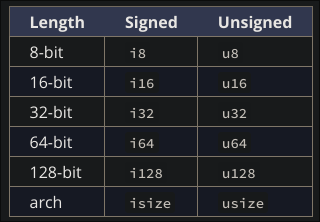
\includegraphics[scale=0.45]{2022-10-19-01:21:45.png}
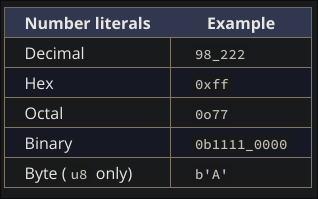
\includegraphics[scale=0.45]{2022-10-19-01:25:19.png}\newline
\textcolor{orange}{The default is i32 integer}
\\
\hline
\end{tabular}
\end{table}
\pagebreak
\begin{table}[ht!]
\begin{tabular}{|m{0.2\linewidth}|m{0.755\linewidth}|}
\hline
Float and double & 
\textcolor{orange}{In rust double is the default floating point type!}\newline
\begin{lstlisting}
let x = 5.5; // has type f64 -> double
let x: f32 = 5.5; // this is a float -> float is f32
\end{lstlisting}
\, \newline 
\textcolor{teal}{Note for calculations, just like in c++ if you do divisions,
make sure you use floats, unless you want truncated values:}\newline
\begin{lstlisting}
let x = 5 / 2;
// x = 2!
let x = 5.0 / 2.0;
// x = 2.5
\end{lstlisting}
\\
\hline
Chars & 
\begin{lstlisting}
fn main() {
    let c = 'z';
    let z: char = 'Z'; // with explicit type annotation
    let heart_eyed_cat = 'emoj';
    // latex might not show it, but you can insert emojis....
}
\end{lstlisting}\\
\hline
Tuples & 
\textcolor{orange}{Tuples are very easy in rust!}\newline
\begin{lstlisting}
    // creating a tuple
    let tup: (i32, f64, u8) = (500, 6.4, 1);

    //accessing a tuple
    let num = tup.1;
    // assigns the first value of tup -> num = 500
    // tup.2 -> 6.4, tup.3 -> 1

    let tup2 = (500, 6.4, 1);
    let (x, y, z) = tup2;
    // assign x = 500, y = 6.4, z = 1
\end{lstlisting}\\
\hline
Arrays & 
\begin{lstlisting}
// creating arrays
let arr = [1,2,3,4,5];
// implicit type and size
let arr2: [i32;5] = [1,2,3,4,5];
// explicit type and size
let arr3 = [3;5];
// creates an array of: [3,3,3,3,3] 5 times the value 3

// accessing arrays -> done just like c++
// arr[0] -> 1
// arr[1] -> 2
// should you go out of bounds, it will panick -> runtime error
\end{lstlisting}\\
\hline
Function Parameters &
\textcolor{orange}{Function parameters are always explicit!}\newline
\begin{lstlisting}
fn some_func(x: i32, y: char) {
    println!("value of {y} is {x}");
}
some_func(5,'h');
\end{lstlisting}\\
\hline
Scopes in rust & 
\begin{lstlisting}
let y = {
        let x = 3;
        x + 1 // no error this works because of the scope!
    }; // it's essentially a return statement!

println!("The value of y is: {y}");
// will print the value 4
\end{lstlisting}\\
\hline
\textbf{Return} & 
\textcolor{orange}{\textbf{In Rust functions can return values implicitly, and it is also used like this!}}\newline
\begin{lstlisting}
fn ret() -> i32 { // you must specify the return like this! i32 for int
5
}
// this function simply returns 5 !!
\end{lstlisting}
\, \newline
\textcolor{teal}{You can still use the return keyword in rust, it is just not needed -> choose a style...}\newline
\textcolor{red}{\textbf{More importantly: the return value MUST be written and it is after an arrow: \emph{->}}}\\
\hline
\end{tabular}
\end{table}
\pagebreak
\begin{table}[ht!]
\begin{tabular}{|m{0.2\linewidth}|m{0.755\linewidth}|}
\hline
Expressions vs Statements &
\textcolor{red}{\textbf{VERY IMPORTANT, rust makes a clear difference between an expression and a statement.}}\newline
\textcolor{orange}{A statement is something like a variable to return in a function, while an expression is something like a function call some\_func()}\newline
\textcolor{red}{\textbf{So, yes, when returning a value you do not put a semicolon at the end!}}\newline
\begin{lstlisting}
fn some_func() -> i32 {
    5 // NO SEMICOLON!!!!!
    5; // WRONG!!!!
}
\end{lstlisting}\\
\hline
If statements & 
\textcolor{orange}{In rust if statements do not need brackets around them, the compiler even tells you about unnecessary brackets!}\newline
\begin{lstlisting}
if x > 5 {
    println!("ping pang");
} else {
    println!("sadly no pang ping");
}
\end{lstlisting}
\, \newline
\textcolor{teal}{There is one more caviat, since rust does not do implicit type conversion if there is data loss, it also doesn't convert integers to booleans!}
\begin{lstlisting}
let x = 5;
if x {
 // doesn't work !!! error implicit cast not allowed!
}
if x != 0 {
 // works
}
\end{lstlisting}\\
\hline
Inline If & 
\textcolor{teal}{You can also write inline if statements to for example assign a value to a variable:}\newline
\begin{lstlisting}
let x = 5;
let y = if x > 6 {4} else {3};
// y now has the value of 3 as x is not greater than 6
\end{lstlisting}\\
\hline
Loops & 
\textcolor{orange}{Prepare for brainfuck, loops in rust are super weird, here an example with comparison to c++}\newline
\textcolor{teal}{Note that this can be done differently with a for loop in c++!}\newline
\begin{lstlisting}
fn main() {                                    void main() {        
    let mut counter = 0;                           int result = 0;
                                                   int counter = 0;
    let result = loop {                            while (true) {
        counter += 1;                                  if (counter == 10) { 
                                                          result = counter * 2;
        if counter == 10 {                             } 
            break counter * 2;                     counter += 1;
        // <<< result = counter * 2 !!!!          }
        }                                      std::cout << "The result is " << result << "\n";
    };                                         }
    println!("The result is {result}");       
}
\end{lstlisting}
\, \newline
\textcolor{orange}{Take a close look at the break counter * 2, this is essentially a return statement from a loop that will be assigned to the variable result.}\\
\hline
Loops with labels &
\textcolor{orange}{Another quirk with loops in rust is that you can assign labels to loops, this is needed to break out of a loop without assigning a value!}\newline
\begin{lstlisting}
let mut counter = 0;
'some_name: loop { // notice the ' at the start !!!!
    if counter == 2 {
        break 'some_name; // break the loop with label some_name
        // this means you can break loops nested loops!!!!
    }
    counter += 1;
}
\end{lstlisting}\\
\hline
While Loops &
\textcolor{teal}{While loops are the same as c++ without the brackets.}\newline
\begin{lstlisting}
let mut counter = 0;
while counter != 3 {
    counter += 1;
    println!({counter});
}
\end{lstlisting}\\
\hline
\end{tabular}
\end{table}
\pagebreak
\begin{table}[ht!]
\begin{tabular}{|m{0.2\linewidth}|m{0.755\linewidth}|}
\hline
For Loops &
\textcolor{teal}{For loops can be used like ranged based for loops in c++ and co.}\newline
\begin{lstlisting}
let x = [1,2,3,4,5];
for element in x {
    println!({element});
}
\end{lstlisting}
\, \newline
\textcolor{orange}{For loops like this for (int i = 0; i < x.size; i++), you write the following:}\newline
\begin{lstlisting}
for number in (1..x.size()).rev() { // x.size == 4
    // instead of x.size you can put any number there !
    println!("{number}!");
}
\end{lstlisting}\\
\hline

\hline
\end{tabular}
\end{table}
\end{document}
